\chapter{Use Cases}
\label{sec:Use_Cases}

In order to assess the suitability of the HR ticket dataset for downstream machine learning applications in HR, we exploit the obtained dataset using as labels the categories of the tickets. \\
The goal of testing different downstream machine learning tasks on the dataset is to show that our dataset is sufficiently rich to enable meaningful learning. \\
All the experiments have been carried out using as training data the dataset generated by the model, whereas the test data used was the tickets collected with the survey. \\ 
One of the main motivations to acquire the survey tickets was to have data that had no biases, or at least biases different from ours. Using a portion of the HR tickets dataset as test data would be meaningless, since the model would not necessarily be tested with data that was outside of the one it had been trained with. On the contrary, achieving good results on a portion of the HR ticket dataset would assert the performance of the models used and not the usefulness of the dataset.

\section{Classification}
Sentence classification is a natural language processing task that involves assigning a predefined category or label to a given sentence. One way to approach sentence classification is to use word embeddings, which are numerical representations of words that capture their meaning and context within a sentence. Word embeddings can be generated using various techniques, such as training a neural network on a large dataset of text or using a pre-trained language model. \\
Once the word embeddings have been generated, you can input them into a classifier along with other features of the sentence, such as its grammatical structure, to make predictions about the sentence's category or label. The classifier uses the word embeddings as input to make predictions about the sentence's category or label. \\
We used two different pre-trained language models: BERT and fastText. We chose BERT because it is a widely used and well-studied model, and our objective was not to find the absolute best classifier, but only to show that the dataset could be used as training data. \\
Instead, we chose fastText to have an option that was CPU-friendly, and that could be trained in a matter of a few minutes. \\
The training data used were the texts of the 16000 tickets that compose the HR ticket dataset, whereas the test data were the survey tickets. The labels were the combination of ticket category and ticket subcategory of each ticket ( Ex. "Life event\_Health issues").


\subsection{FastText Classifier}
FastText is a library developed by Facebook AI Research that provides a set of training algorithms for supervised learning of word embeddings from raw text and also can be used to build and train supervised text classification models. \\
FastText creates word embeddings using a combination of character n-grams and word n-grams. To do this, fastText first breaks each word in the training text into its constituent character n-grams. For example, the word "cat" might be broken into the character n-grams "c", "ca", "cat", "a", "at", and "t". These character n-grams are then used to generate vectors. The word embeddings are calculated as the sum of their n-gram vectors. \\
To learn the embeddings of these n-grams, fastText uses a skip-gram model, which is a type of model that maximizes the probability of observing a word given its context, or in other words its surrounding words. By using this approach, fastText is able to learn high-quality word embeddings that capture the syntactic and semantic information of words. \\
The fastText classification uses the fastText embeddings as input to the model, and in particular:
\begin{algorithm}
    \caption*{fastText Classification}
    \begin{algorithmic}[1]
      \State Words representation are averaged into a text representation
      \State The text representation is fed to a linear classifier
      \State The output of the linear classifier is given as input to a softmax function to compute the probability distribution over a set of predefined classes
    \end{algorithmic}
\end{algorithm}


\subsection{BERT classifier}
BERT (Bidirectional Encoder Representation from Transformers) is a model developed by Google AI based on the transformers architecture. BERT was trained on a large corpus on two different tasks: Masked Language Modeling and Next Sentence Prediction. \\
Through the use of MLM, in the training phase, 15\% of the tokens in a sentence are obscured and BERT can then be utilized to utilize the surrounding words in both directions to predict the masked tokens, facilitating bidirectional learning from the text. \\
On the other hand, NSP helps the model understand the relationships between sentences. Specifically, in the training phase, 50\% of the examples are actually successive sentences, while in the other 50\% of the cases this condition is not respected. \\
BERT is quite straightforward to fine-tune, we just need to plug in the necessary layers at the top of the BERT architecture and fine-tune for a sufficient number of epochs the model end-to-end. \\
The first token of a BERT embedding is the [CLS] token, which is a special token that acts as an aggregate representation of the sentence. The final embedding of the [CLS] token is used as input for the classification task. The most simple method, which is also the method used by the BERTForSequenceClassification class by HuggingFace, is to take the embedding of the [CLS] token at the last hidden layer and fed it to a single layer of a feed-forward network. The layer of the feed-forward network will have n input, where n is the dimension of the embedding of a token, and m output, where m is the desired number of outputs. \\
The final model is shown in \autoref{fig:bert_class}
\begin{figure}[h] 
  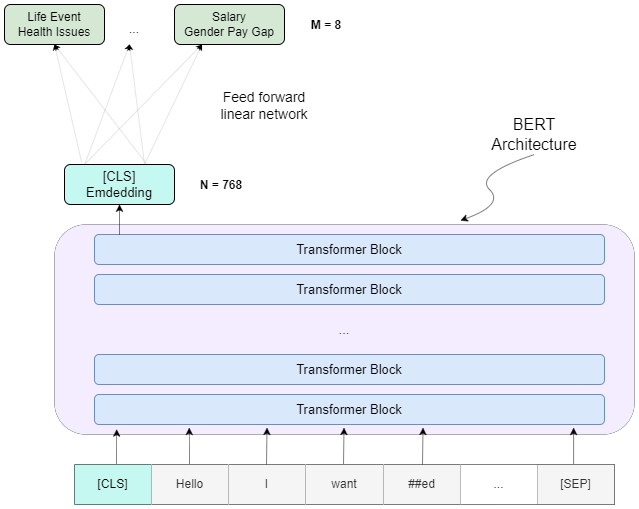
\includegraphics[width=\textwidth]{images/bert_class.drawio.png}
  \caption{Schema of BERT classification}
  \label{fig:bert_class}
\end{figure}

\subsection{Results}
In this section we show the results of the classification experiments. We want to reiterate that the point of the experiments was not to get the best possible results, therefore the models were not trained for a large number of epochs and we did not try an excessive number of possible hyperparameters.
The hyperparameters tried are shown in \autoref{table:hyp_fasttext} and \autoref{table:hyp_bert}. If a hyperparameter is not shown in the table it means we have used its default value. \\
The technique used for finding the optimal hyperparameters is Grid Search, which means we have trained and tested the models for each combination of all the chosen values of the hyperparameters to determine the hyperparameters' set which achieves the best results.

\begin{table}[h]
  \begin{tabular}{|l|l|}
  \hline
  Size of context window (ws)                   & 5      \\ \hline
  epochs                                        & 20     \\ \hline
  minimal number of word occurrences (minCount) & 1      \\ \hline
  max length of word ngram (wordNgrams)         & 3      \\ \hline
  learning rate (lr)                            & 0.5    \\ \hline
  learning update rate (lrUpdateRate)           & 100    \\ \hline
  sampling threshold (t)                        & 0.0001 \\ \hline
  \end{tabular}
  \caption{Hyperparameters fastText}\label{table:hyp_fasttext}
\end{table}

\begin{table}[h]
  \begin{tabular}{|l|l|}
  \hline
  epochs           & {[}3, 5{]}                              \\ \hline
  learning rate    & {[}1e-05, 5e-04, 1e-04, 5e-05, 5e-06{]} \\ \hline
  weight decay     & {[}0.001, 0.01, 0.05{]}                 \\ \hline
  train batch size & {[}8, 16{]}                             \\ \hline
  warmup steps     & 500                                     \\ \hline
  \end{tabular}
  \caption{Hyperparameters BERT}\label{table:hyp_bert}
  \end{table}

%TODO: add results
As we expected, fastText performs worse than BERT, achieving an $f_1$ score of only 0.41. \\
On the other hand, the BERT classifier with hyperparameters\begin{itemize}
  \item epochs: 5
  \item learning rate: 5e-05
  \item weight decay: 0.001
  \item train batch size: 8
  \item warmup steps: 500
\end{itemize}
achieved an $f_1$ score of 0.78. We show also the confusion matrix( \autoref{fig:conf_matrix_bert_class} ) to highlight how the majority of errors come from two sub-categories that belong to the same category, in particular, "Gender wage gap"-"Salary raise" and "Personal issues"-"Health issues". In some way, this validates our initial decision on the taxonomy of the tickets.
\begin{figure}[h] 
  \centering
  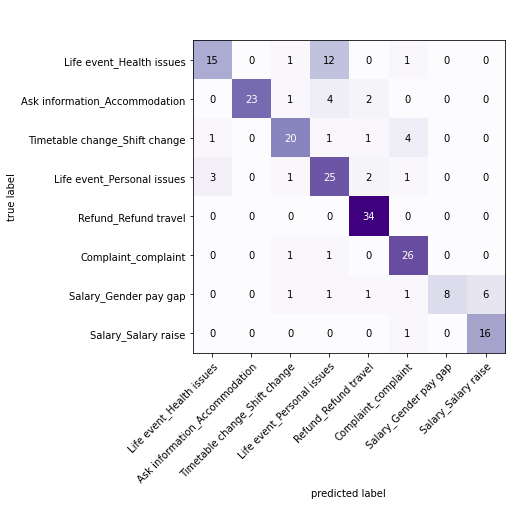
\includegraphics[width=0.8\textwidth]{images/conf_matrix_bert_class.png}
  \caption{Confusion matrix of Ticket classification with BERT}
  \label{fig:conf_matrix_bert_class}
\end{figure}    

\section{Anonymization}

Anonymization of personal data refers to the process of removing personally identifiable information (PII) from data sets so that the individuals represented in the data cannot be identified. This is accomplished by either completely removing or replacing identifiable data with generic values. The purpose of anonymization is to protect the privacy of individuals while still allowing the data to be used for legitimate purposes. \\
Most of the recent implementations of anonymization work by masking the personal information of a person, such as names and surnames, telephone numbers, addresses, credit card numbers and so on. \\
One of the most famous libraries for anonymization is Presidio, developed by Microsoft. Presidio exploits pattern recognition with regex and Named Entity Recognition to find all the personal information and mask them. \\
The main disadvantage of such techniques is that often the personal subject can be identified through the so-called quasi-identifiers, that more often than not are not masked.
\\Here reported some examples that are not masked by Presidio:\\ \\
Original sentence
\begin{adjustwidth}{1cm}{}
    The new intern at my office, the one with red hair, caught covid last week 
\end{adjustwidth}
Sentence redacted by Presidio
\begin{adjustwidth}{1cm}{}
    The new intern at my office, the one with red hair, caught covid \textless DATE\_TIME \textgreater
\end{adjustwidth}
Original sentence
\begin{adjustwidth}{1cm}{}
    The boss of the HR department has made some weird comments about how I dress
\end{adjustwidth}
Sentence redacted by Presidio
\begin{adjustwidth}{1cm}{}
    The boss of the HR department has made some weird comments about how I dress 
\end{adjustwidth}
Our new approach exploits a Sequence to Sequence model called T5
T5 is a model released by Google in 2019, it is a standard encoder-decoder transformer that, unlike BERT, always returns strings as outputs. This is why it is called a sequence-to-sequence model. \\
T5 is a unified model that can be applied for many downstream tasks, such as sentiment analysis, sentence completation, question answering\dots\\
In T5 architecture there are \textit{adapted layers} after each feed-forward layer, whose scope is to diminish the number of parameter updates for each fine-tuned model. In fact, \textit{adapted layers} are dense-ReLU-dense blocks that are designed so that their input dimensionality and output dimensionality are equal. This lets us insert them into the Transformer architecture without other changes. When fine-tuning for each different task, only the \textit{adapted layers} and the normalization layers will be updated. This results in a considerable reduction of parameter updates.\\
We followed a few-shot learning approach with T5. Rather than relying on a large amount of training data to allow a pre-trained model to adjust to a given task accurately, few-shot learning employs the use of a few examples to direct the training of a machine learning model with very minimal data. \\
For each category of tickets, we wrote 10 examples of "anonymized" tickets, where we removed all personal information and information that could be retraced to the original writer, maintaining only information that could be useful for analysis purposes.
Here are a couple of examples:\\ \\
Original sentence:
\begin{adjustwidth}{1cm}{}
    Dear Sir/Madame, I cannot stand anymore this discrimination and prejudice against French people at work
\end{adjustwidth}
Anonymization used for few-shot learning:
\begin{adjustwidth}{1cm}{}
    The employee is filling a complaint for discrimination based on nationality 
\end{adjustwidth}
Original sentence:
\begin{adjustwidth}{1cm}{}
    Hello, my name is Zacaredas Pinilla and I work at Laguna-Franco Spain. I am having trouble finding accommodation in the Algeciras area so if you could help me with this matter it would be greatly appreciated
\end{adjustwidth}
Anonymization used for few-shot learning:
\begin{adjustwidth}{1cm}{}
    The employee is asking for help finding an accommodation
\end{adjustwidth}
\begin{figure}[h] 
    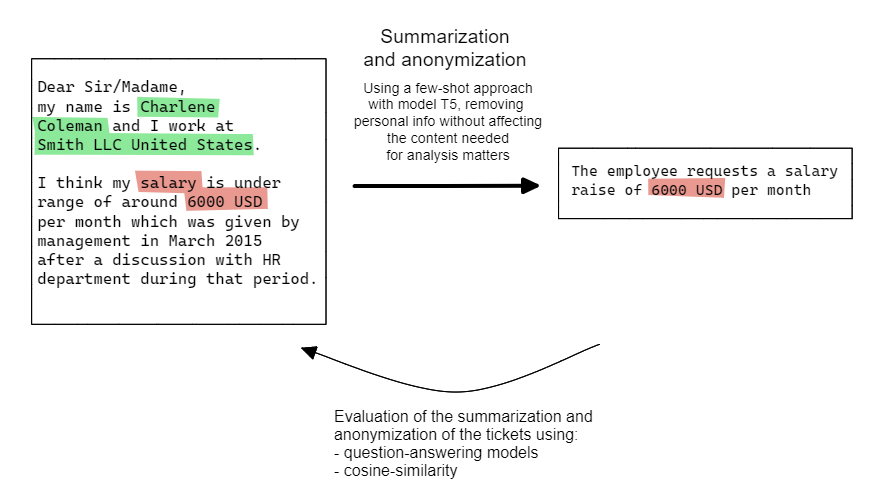
\includegraphics[width=\textwidth]{images/ticket_anonymization_schema.png}
    \caption{Schema of Ticket Anonymization}
    \label{fig:schema_ticket_anonymization}
\end{figure}    
To evaluate the goodness of anonymization and how much of the information has remained after the anonymization we have used three different methods:
\begin{itemize}
    \item \textbf{QAGS}: Questions Answering and Generation for summarization
    \item \textbf{SUMMAQA}: Unsupervised metric for reinforced summarization model 
    \item \textbf{Cosine Similarity}
\end{itemize}  
These models were created originally to evaluate the goodness of a summarization, we have adapted them to be used for evaluating our anonymization. \\
The first two methods follow the same philosophy: they generate questions to ask both the original version and the anonymized version of the tickets, looking if the answers are coherent. We call them Questions and Answers models.
However they have few key differences. SummaQA do not create natural sentence questions but uses as questions the masked version of the sentences. Instead QAGS create natural language questions using a pre-trained model.
\subsection*{QAGS}
QAGS is an automatic evaluation protocol that is based on the assumption that if we reply to questions considering as factual bases the summary and the source, we can determine if the summary/anonymization is consistent with its source by comparing the answers. \\
QAGS works like this:
\begin{algorithm}
    \caption*{QAGS}
    \begin{algorithmic}[1]
      \State A BART model is fine-tuned for question generation: the model receives both the answers and the source article from the NewsQA dataset and is trained to maximize the likelihood of the paired question
      \State At test time, named entities and noun phrases are extracted from the context using spaCy and are considered as answers candidates. The summary is used as the context.
      \State The BART model generates question based on the summary and its entities
      \State A BERT model is fine-tuned for Question Answering on the SQuAD dataset
      \State We answer with the help of the fine-tuned BERT model the questions generated beforehand using both the source article and the summary to get two sets of answers. 
      \State We compare the corresponding answers using an answer similarity metric, and we get a final score averaging the answer similarity metric (f1 score) over all questions
    \end{algorithmic}
\end{algorithm}

\subsection*{SUMMAQA}
SUMMAQA works similarly to QAGS, the main difference is that there is not a generative model to create the questions, in particular:
\begin{algorithm}
    \caption*{SUMMAQA}
    \begin{algorithmic}[1]
      \State We find all the entities in the source text (the original ticket) with Spacy
      \State Create one sentence (which will be our question) for each entity. We keep only the sentence in which the entity is if there are more sentences. The entity will be masked. Ex: "Yesterday I went to Paris" becomes "Yesterday I went to [MASK]"
      \State The MASKED entities will be the True labels when calculating the metrics
      \State We answer to the questions generated before using a fine-tuned version of BERT model, using both the source and the summarization/anonymization as contexts
      \State We compare the answers and calculate the f1 score for both contexts
    \end{algorithmic}
\end{algorithm}
\subsection*{Cosine Similarity}
We measured the cosine similarity between sentence embeddings of original text and summarization. The sentence embeddings used were calculated using Sentence-BERT, a modified version of the pretrained BERT network that uses siamese networks to obtain more meaningful embedding of the sentence, compared to getting the embedding of the [CLS] token or to average all the other emeddings.

%TODO: maybe put little schema of Siamese network of sentence-bert

\begin{figure}[h] 
    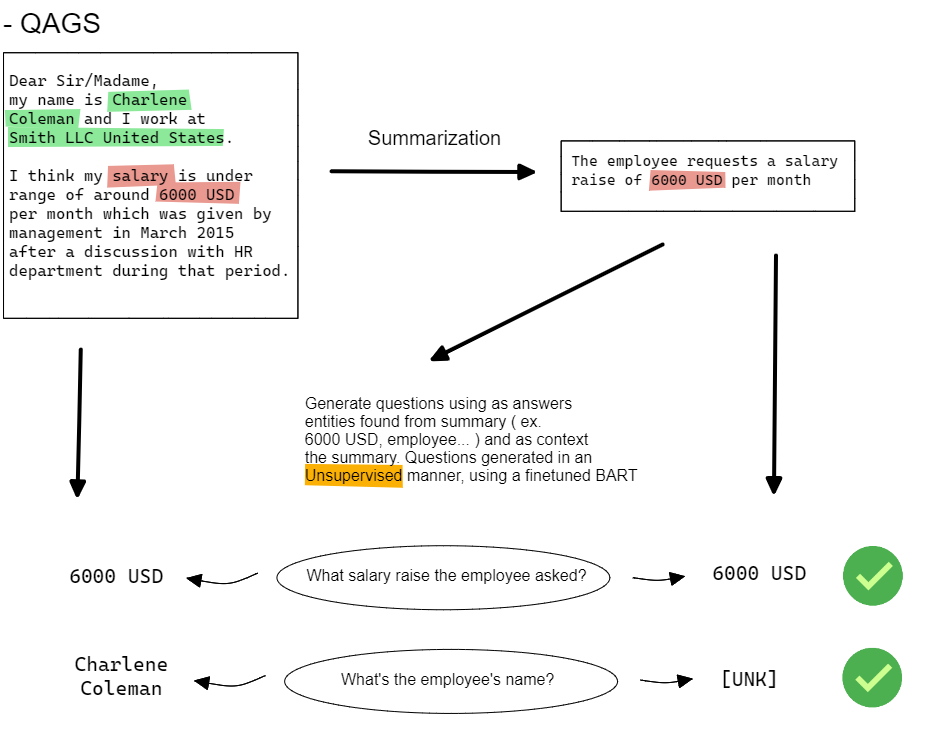
\includegraphics[width=\textwidth]{images/qa_models_qags.png}
    \caption{Schema of QAGS}
    \label{fig:schema_qags}
\end{figure}    

\begin{figure}[h] 
    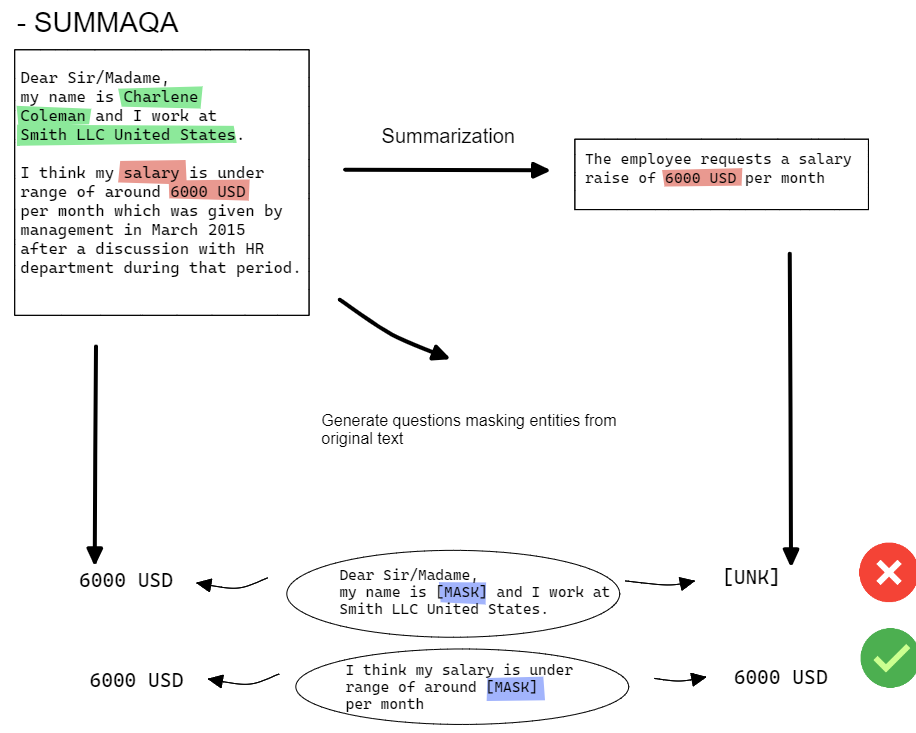
\includegraphics[width=\textwidth]{images/qa_models_summaqa.png}
    \caption{Schema of SUMMAQA}
    \label{fig:schema_summa_qa}
\end{figure}    

\begin{figure}[h] 
    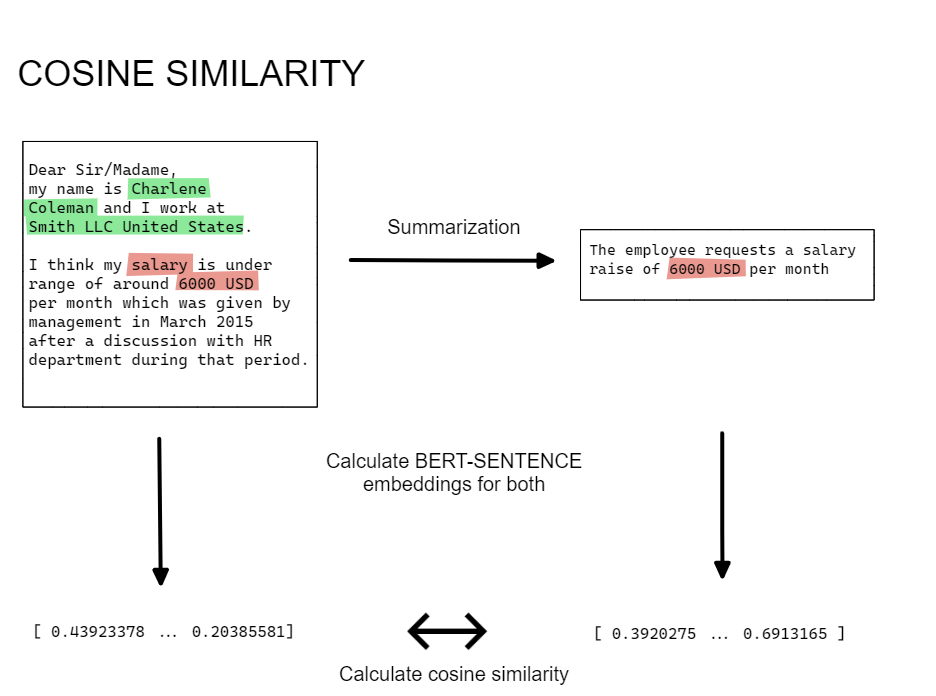
\includegraphics[width=\textwidth]{images/cosine_similarity.png}
    \caption{Schema of Cosine Similarity for }
    \label{fig:schema_cosine_similarity}
\end{figure}    





\clearpage
\section{Named Entity Recognition}
\label{sec:ner}
Named entity recognition is the process of automatically identifying and classifying named entities in a text. This can include identifying and categorizing named entities such as people, organizations, locations, and so on. \\
NER systems might be used to automatically extract information from a large collection of documents, such as identifying all mentions of specific named entities or analyzing the relationships between different named entities. \\

\subsection{Weak labeling}
During the creation of the ticket, we tried to automatically save also the entities of the ticket. With entities, we do not mean the classical entities used for NER, but the original variables specific to a ticket's category (complete list in \autoref{table:categoriesTable}). \\
Finding the entities in the prompt is trivial, since the positions are fixed in the template, and the filling operation is managed by us. \\
Example:
\begin{adjustwidth}{1cm}{}
    From: \$\{email\} \\
    To: \$\{company email\} \\
    First name: \$\{first name\}\\
    Last name: \$\{last name\}\\
    Company: \$\{company\}\\
    Date: \$\{ticket date\}
    Date start absence: \colorbox{yellow!30}{\$\{date\_start\_absence\}}\\
    Reason absence: \colorbox{yellow!30}{\$\{reason\_absence\}}\\
    Subject: Request for sick leave for \colorbox{yellow!30}{\$\{days\}}    
\end{adjustwidth}
Though the template and prompt serve as our starting point to generate the actual ticket text, it is only this latter part that would be present in a real ticket. Identifying the locations of the entities is not straightforward since I usually provide only the initial information and a limited template, with the rest of the generation being done by GPT. \\
Once the ticket is generated, to find the entities in the generated text I use 2 different approaches:
\begin{itemize}
    \item Exact match
    \item Heuristics
\end{itemize}
The exact match is straight-forward, it just looks for the exact same words in the generated text, and if the word/words are found, the entity is added to the list of entities of the ticket
However this method often does not work, since GPT could use only part of the entity ( Ex: "A medical consultation" is in the text as "a consultation") or slightly alter the entity ( ex: 01/10/1998 $\rightarrow$ the first of October of 1998 ) \\
This is the reason why we implemented manually a set of different rules to find modified versions of the original entity in the text. These versions do not cover every possible case, since they are hard-coded by us from experience and by looking at how GPT behaves, this is why we called this approach "Heuristics". \\
Some of these heuristics are:
\begin{itemize}
    \item Check not only the full entity, but also subsets of it removing stopwords\\
    Example: \\
    reason\_of\_absence: "An Urinary Tract Infection" $\rightarrow$
                 \begin{itemize}
                    \item "Urinary Tract Infection"
                    \item "Urinary Tract"
                    \item "Tract Infection"
                    \item "Urinary"
                    \item "Tract"
                    \item "Infection"
                \end{itemize}
    \item Check all the possible version of a percentage text\\
    "5\%", "5 \%", "5.0\%", "5 percent", \dots
    \item Check different formats of date\\
    MM/DD/YYYY, DD/MM/YYYY, "First of October", "1st of October", \dots

\end{itemize}
With this method, we were able to identify entities in only 6272 tickets out of the total 16000 tickets. The complete list of all the entities found is shown in \autoref{table:entities_found_heuristics}.

\begin{table}[h]
    \centering
    \begin{tabular}{|l|l|l|l|}
    \hline
    duration                 & 1016 & increase\_in\_percentage & 539 \\ \hline
    location                 & 1411 & work\_title & 33 \\ \hline
    date                     & 70   & wage\_gap & 421 \\ \hline
    work\_shift              & 70   & number\_of\_days & 982 \\ \hline
    reason\_of\_change       & 7    & date\_start\_absence & 3 \\ \hline
    to\_who                  & 1221 & description\_life\_event & 1214 \\ \hline
    reason                   & 1119 & date\_travel & 112 \\ \hline
    complaint                & 106  & airport & 28 \\ \hline
    salary                   & 376  & & \\ \hline
    \end{tabular}
    \caption{Entities found with heuristics}\label{table:entities_found_heuristics}
\end{table}

\subsection{Classical NER}
\label{sec:classical_ner}
Token classification is a common technique used in NER to identify and classify named entities in a text. In token classification, the text is first divided into individual tokens, which are typically words or phrases. The model then predicts a label for each token, indicating the type of named entity it represents.\\
To assign the labels to the tokens we used the BIO(Beginning, Inside, Outside) format, where the B tag is used for the first token of an entity, the I tag for the rest of the tokens of the entity and lastly the O tag is used for the tokens that do not belong to any entities. \\
Example:
\begin{adjustwidth}{1cm}{}
    Alex B-PER\\
    is O\\
    going O\\
    to O\\
    Los B-LOC\\
    Angeles I-LOC\\
    in O\\
    California B-LOC
\end{adjustwidth}
The labels assigned to each token are then used for a token classification task, using a RoBERTa model and the Spacy training pipeline. \\
We used the default Spacy parameters for the training. \\
The survey tickets, used as always as our test set, were manually labeled by ourselves. \\
%TODO: maye put image of schema token classification for NER
The results were not satisfying, we achieved a $f_1$ score of 0.34 on the exact matching and a $f_1$ score of 0.45 on the partial matching. When the model finds the correct entity for all the tokens and only the tokens of an entity, it's considered an exact matching. Whereas, when the model finds the correct entity for only a subset of the token of an entity, then is considered a partial match\\
Example exact match:
\begin{adjustwidth}{1cm}{}
    to O\\
    Los LOC\\
    Angeles LOC\\
    in O\\
\end{adjustwidth}
Example partial match:
\begin{adjustwidth}{1cm}{}
    to O\\
    Los LOC\\
    Angeles O\\
    in O\\
\end{adjustwidth}
The main problem we encountered was that the NER model was not able to recognize the different entities of the same type depending on the context. For example, the model could not recognize the difference between a date of start absence ( entity of request of time off due to health reasons) and a date of travel ( entity of request of refund for travel).

\subsection{Our approach to NER}
\label{sec:ner_nc}
To overcome the limits of the first approach, we developed a new approach based on transfer learning and sentence classification. \\
The main intuition behind the new approach is to use the pre-trained spacy NER model and exploit the entities found by the base model to extract our entities. \\
First of all, we build a dictionary of the matchings between entities of Spacy and our entities. We decided to work on a subset of our entities and not consider all the entities that did not have a clear matching with Spacy entities. In \autoref{table:entities_match} we show all the matchings. 
\begin{table}[h]    
    \resizebox{\textwidth}{!}{
    \setlength\extrarowheight{18pt}
    \begin{tabular}{|l|l|}
    \hline
    Category                       & Entities matching                                              \\ \hline
    Ask information\_Accommodation & \shortstack[l]{\{"location": "GPE", \\"duration": "DATE"\}}                       \\ \hline
    Life event\_Health issues      & \shortstack[l]{\{"date\_start\_absence": "DATE", \\"number\_of\_days": "DATE"\}} \\ \hline
    Refund\_Refund travel          & \shortstack[l]{\{"date\_travel": "DATE",\\ "location": "GPE"\}}                  \\ \hline
    Salary\_Gender pay gap         & \{"wage\_gap": "PERCENT"\}                                     \\ \hline
    Salary\_Salary raise           & \shortstack[l]{\{"increase\_in\_percentage": "PERCENT",\\"salary": "MONEY"\}}    \\ \hline
    Timetable change\_Shift change & \{"date": "DATE"\}                                             \\ \hline
    \end{tabular}}
    \caption{Matching of our entities with Spacy entities}\label{table:entities_match}
\end{table}
Then, we scan our dataset and look, for all categories, the entities shown in \autoref{table:entities_match}. If we find an entity not present in the table, it is filtered out. For each entity, we will have an array of the type [ ENTITY, START\_CHAR, END\_CHAR ] (\autoref{fig:ticket_NER_NC_1}).\\
\begin{figure}[h] 
    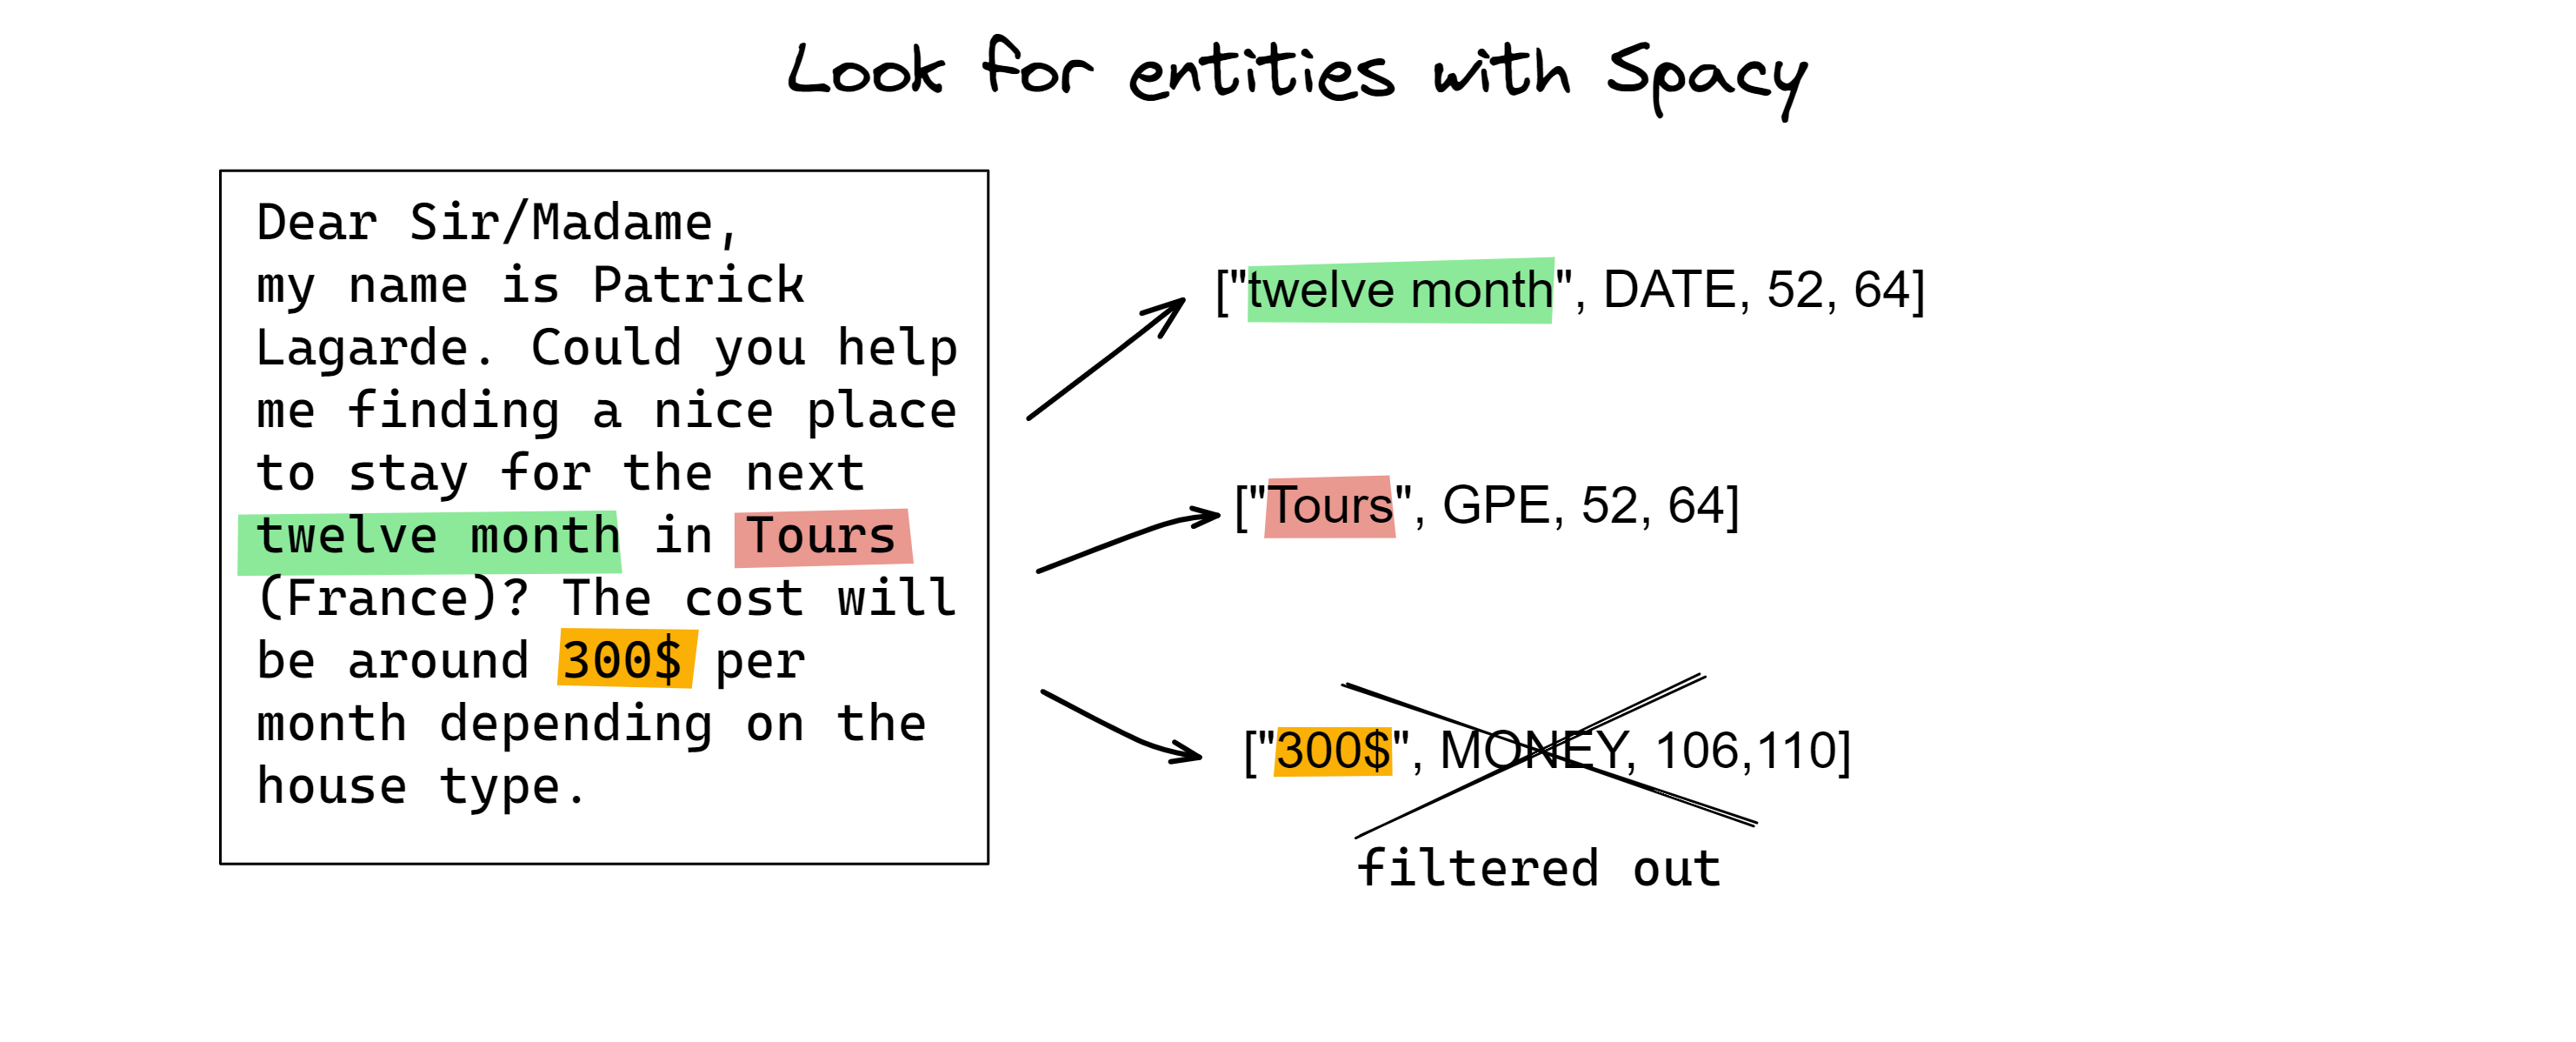
\includegraphics[width=\textwidth]{images/NER_nc_1.png}
    \caption{Ticket NER preprocessing part 1}
    \label{fig:ticket_NER_NC_1}
\end{figure}    
After that, we tokenize the text of all the tickets and we look up for each ticket its entities' tokens. Then for each entity, we save the indexes of the corresponding tokens, so for example if the entity "twelve months" is split into two tokens "twelve" and "month", which are the $22^{nd}$ and $23^{rd}$ tokens of the text, then we will save ["twelve months", DATE, [22,23]]. \\
We also had to manage the case in which a token is not present in the tokenizer vocabulary, so is split into sub-tokens. We took advantage of the fact that if a word is split into two or more words the new tokens will have the prefix "\#\#". \\
The number of tokens for each entity can vary, for practical reasons in the training phase we set the maximum number of tokens to $N=50$ (\autoref{fig:ticket_NER_NC_2}).
\begin{figure}[h] 
    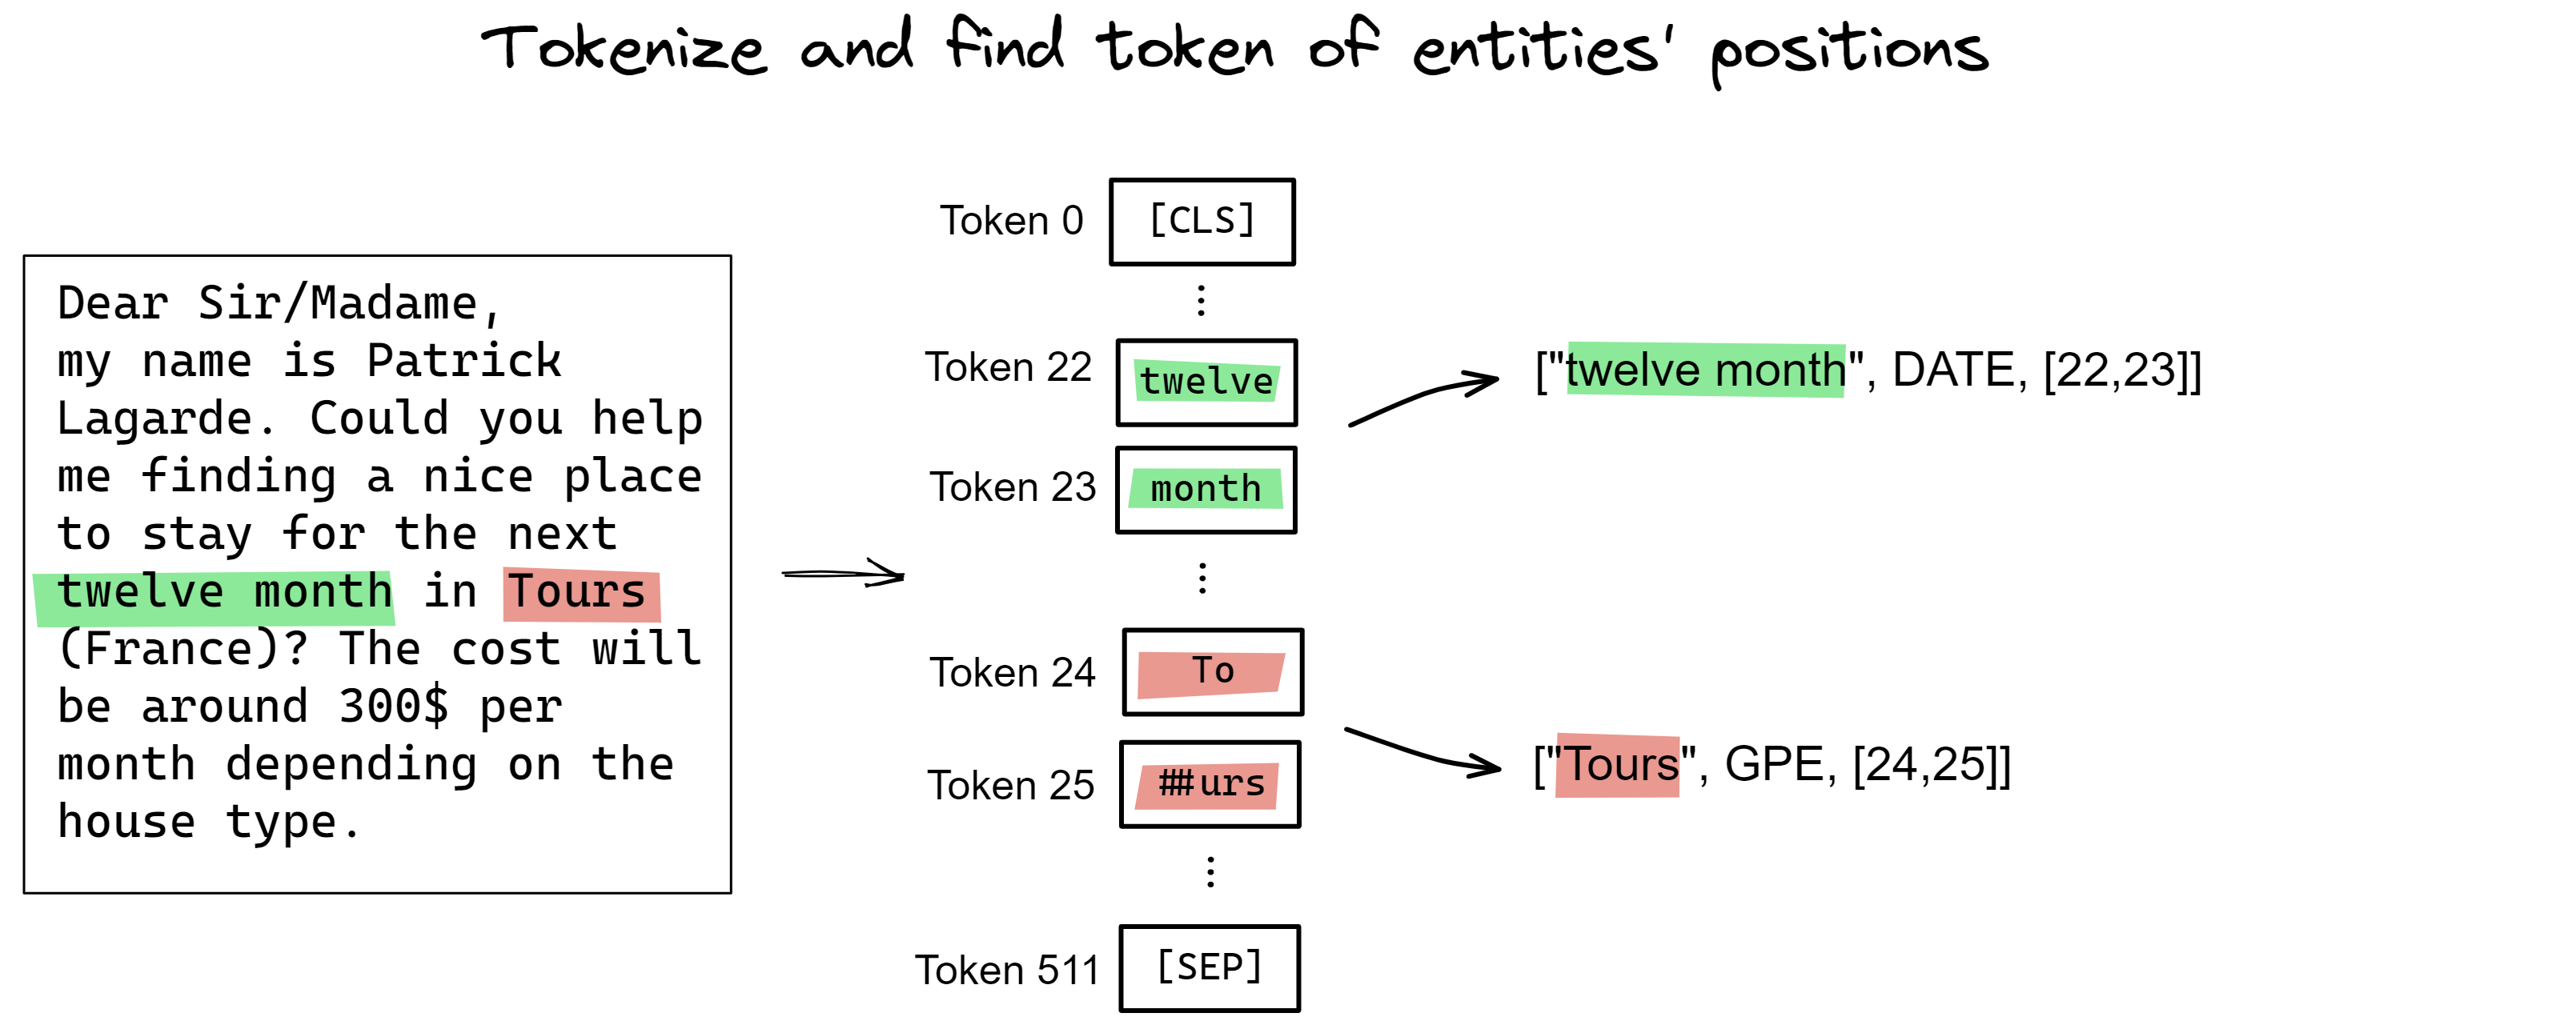
\includegraphics[width=\textwidth]{images/NER_nc_2.png}
    \caption{Ticket NER preprocessing part 2}
    \label{fig:ticket_NER_NC_2}
\end{figure}    
Now we have all we need for the training. The base architecture is a \textit{bert-base-cased} model, which we modified on the last layer. \\
In the training phase, we pass to the BERT model at each step the tickets' texts and their entities with the indexes of the matching tokens. For each entity of the ticket, there will be a training record. The ticket will be unpacked into 512 tokens, and each token will be processed by the BERT architecture (same architecture as the classifier \autoref{fig:bert_class}). \\
At the last layer, instead of passing the [CLS] token to a classifier, we concatenate the [CLS] token with the average of all the embeddings of the tokens of the current entity. This is the reason why we preprocessed the dataset to find the indexes of the tokens' indexes for the entities. In BERT base each token has a dimension $d=768$, so the input of the last feed forward neural network will be $N=1536$. The output dimension will be $M=10$ (\autoref{fig:ticket_NER_NC_3}). The labels of the training are the combination of the ticket category and the entity, since for each entity found in a ticket we generate a record ( For example if there are 3 entities in a ticket, there will be 3 records in the training set with the same ticket text, but that will have a different token embedding for the classification in the last layer and they will have different labels)\\
\begin{figure}[h] 
    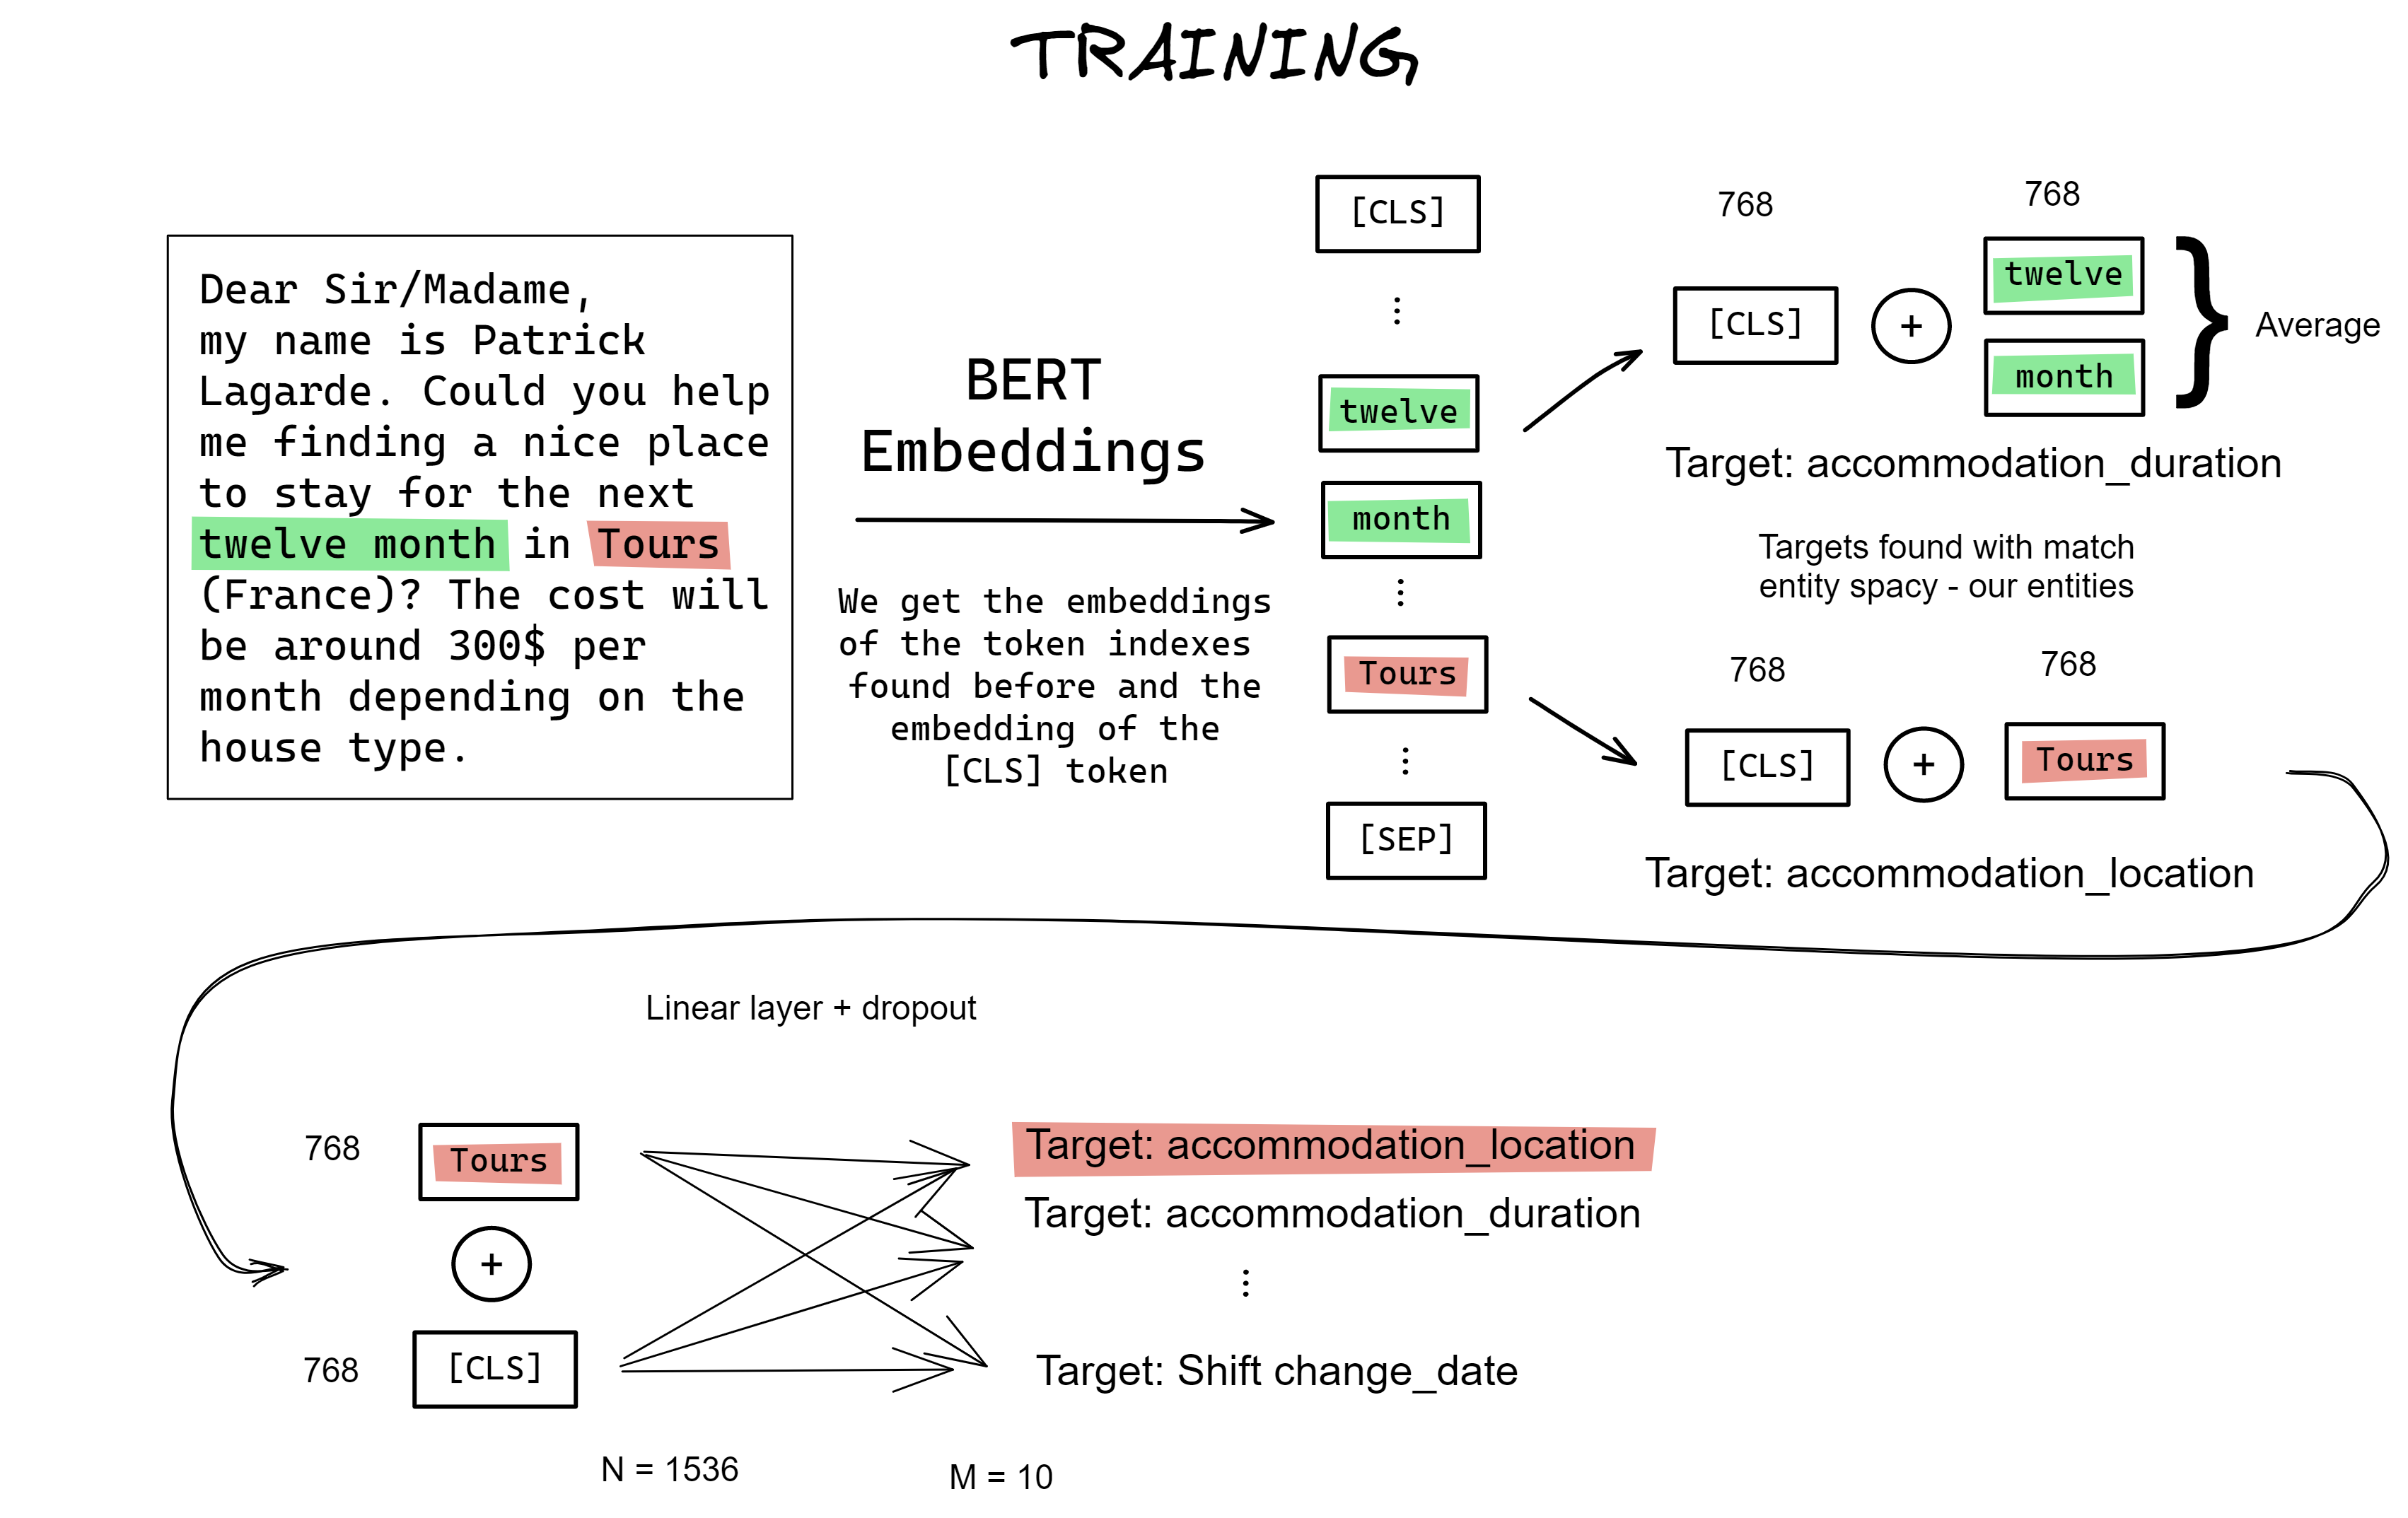
\includegraphics[width=\textwidth]{images/NER_nc_3.png}
    \caption{Ticket NER training}
    \label{fig:ticket_NER_NC_3}
\end{figure}
At test time, for each ticket in the test set, we analyze it with Spacy and we find all the entities. Then we filter the entities: we cannot filter based on the label, since at test time in theory we do not know the label of the tickets. Therefore we filter the entities based on the list of all entities used in all tickets' categories. \\
Then, as in the training phase, for each entity we build a new record composed of the output of the [CLS] token through the model architecture and of the average of the tokens' embeddings. \\
For each ticket in the test set we obtain a prediction of its category combined with the entity currently analyzed. 
\subsubsection*{Results}
We are able to achieve way better results with the new method that combines a ticket classifier with a NER model. On the test set we achieve a $f_1$ score of 0.96. \\
In \autoref{fig:ticket_NER_NC_conf_matrix} we show the confusion matrix of the classification. \\
We believe that we are able to achieve such good results because there are few entities that are shared between more categories, and the union of the information of the ticket ([CLS] token) and the information of the entity makes it easy for the model to distinguish both the category and the entity.
\begin{figure}[h] 
    \centering
    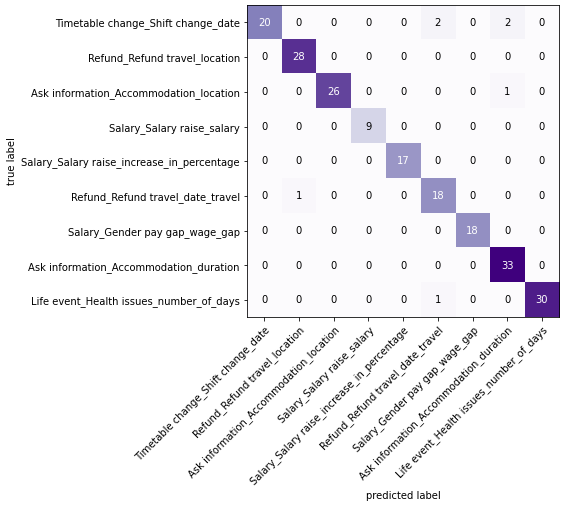
\includegraphics[width=0.8\textwidth]{images/conf_matrix_ner_nc.png}
    \caption{Ticket NER confusion matrix}
    \label{fig:ticket_NER_NC_conf_matrix}
\end{figure}   

